\documentclass[tikz,border=8pt]{standalone}
\usepackage{tikz}
\usetikzlibrary{arrows.meta,positioning,calc,backgrounds,fit,shapes.geometric}
\usepackage[scaled=0.92]{helvet}
\renewcommand{\familydefault}{\sfdefault}
\usepackage{amsmath,amssymb}
\definecolor{ink}{HTML}{262624}
\definecolor{mute}{HTML}{8A8984}
\definecolor{line}{HTML}{BDBBB5}
\definecolor{acc}{HTML}{2A78D6}
\definecolor{accbg}{HTML}{F1F6FD}
\tikzset{
  >={Latex[length=2.2mm]},
  every node/.style={text=ink},
  b/.style={draw=line, fill=white, rounded corners=2pt, align=center, inner sep=6pt,
            minimum height=10mm, text width=#1, font=\small},
  b/.default=40mm,
  a/.style={b=#1, draw=acc, fill=accbg},
  a/.default=40mm,
  t/.style={font=\footnotesize, text=mute, align=center},
  e/.style={->, draw=mute, line width=0.6pt},
  ea/.style={->, draw=acc, line width=0.9pt},
  eh/.style={->, draw=acc, line width=0.9pt, dash pattern=on 3pt off 2pt},
}

\begin{document}
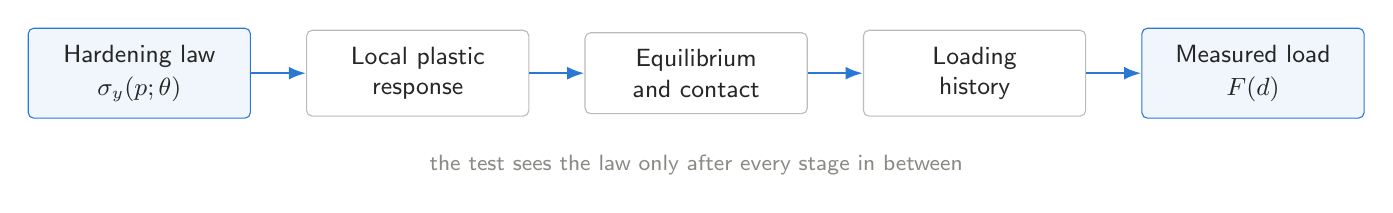
\begin{tikzpicture}[node distance=7mm]
\node[a=24mm] (a) {Hardening law\\[1pt] $\sigma_y(p;\theta)$};
\node[b=24mm, right=of a] (b) {Local plastic\\ response};
\node[b=24mm, right=of b] (c) {Equilibrium\\ and contact};
\node[b=24mm, right=of c] (d) {Loading\\ history};
\node[a=24mm, right=of d] (e) {Measured load\\[1pt] $F(d)$};
\draw[ea] (a) -- (b); \draw[ea] (b) -- (c); \draw[ea] (c) -- (d); \draw[ea] (d) -- (e);
\node[t, below=4mm of c] {the test sees the law only after every stage in between};
\end{tikzpicture}
\end{document}
